\section{最终实验结果与结论}
\subsection{冻结参数流上的精度与触发行为}
最终汇总记录完成了三个网格、每个网格三次重复，共九次有效运行，缺失及无效运行数均为零。每次重复使用同一冻结的 256 个参数；下列精度和轨迹在三次重复中一致，因此每个网格的精度样本量仍为 256，而不是 768。前 24 次查询只是同一序列的前缀，不是另一组测试。这些参数未参与初始建模与选秩；自适应评价则允许按顺序使用当前已付费执行的 FOM 回退解更新基，并将状态传给后续查询。它属于在线顺序评价，不是全程冻结模型的测试；每次计时重复重置全部学习状态，事后参照真解不作为免费预测接口。

\begin{table}[htbp]
\centering\small
\caption{256 次查询的实际输出误差。固定模型使用快速 $r=8$ POD；超标阈值为 $10^{-3}$。}
\label{tab:final-accuracy}
\begin{tabular}{rlrrrr}
\toprule
$n$ & 方法 & 最大场误差 & 最大热点值误差 & 场超标数 & 热点超标数\\
\midrule
24 & 固定 POD & $1.972\times10^{-3}$ & $1.453\times10^{-4}$ & 6 & 0\\
24 & 自适应 POD & $1.270\times10^{-6}$ & $1.132\times10^{-8}$ & 0 & 0\\
48 & 固定 POD & $2.211\times10^{-3}$ & $1.471\times10^{-4}$ & 6 & 0\\
48 & 自适应 POD & $2.967\times10^{-7}$ & $1.043\times10^{-9}$ & 0 & 0\\
96 & 固定 POD & $2.342\times10^{-3}$ & $1.470\times10^{-4}$ & 7 & 0\\
96 & 自适应 POD & $1.203\times10^{-7}$ & $7.415\times10^{-10}$ & 0 & 0\\
\bottomrule
\end{tabular}
\end{table}

完整组装与快速固定 POD 的误差仅有浮点量级差异，场超标计数相同。表\ref{tab:final-accuracy}说明，仅监测热点值会遗漏本次出现的温度场失准。自适应方案在这些有限测试上均达标，但其触发质量必须单独评价：三个网格分别触发 15、15、17 次实际 FOM 回退，全部成功增广，最终秩分别为 23、23、25；这 47 次触发的\textbf{当前回退前 ROM 场误差均已达标}，因此全部属于按既定定义统计的误触发。不存在漏报的观测也不能证明判别器最优。较保守的触发提前增加了基向量，后续精度改善伴随这些基更新出现，不能把每次触发描述为发现了真实超标。

\begin{figure}[htbp]
\centering
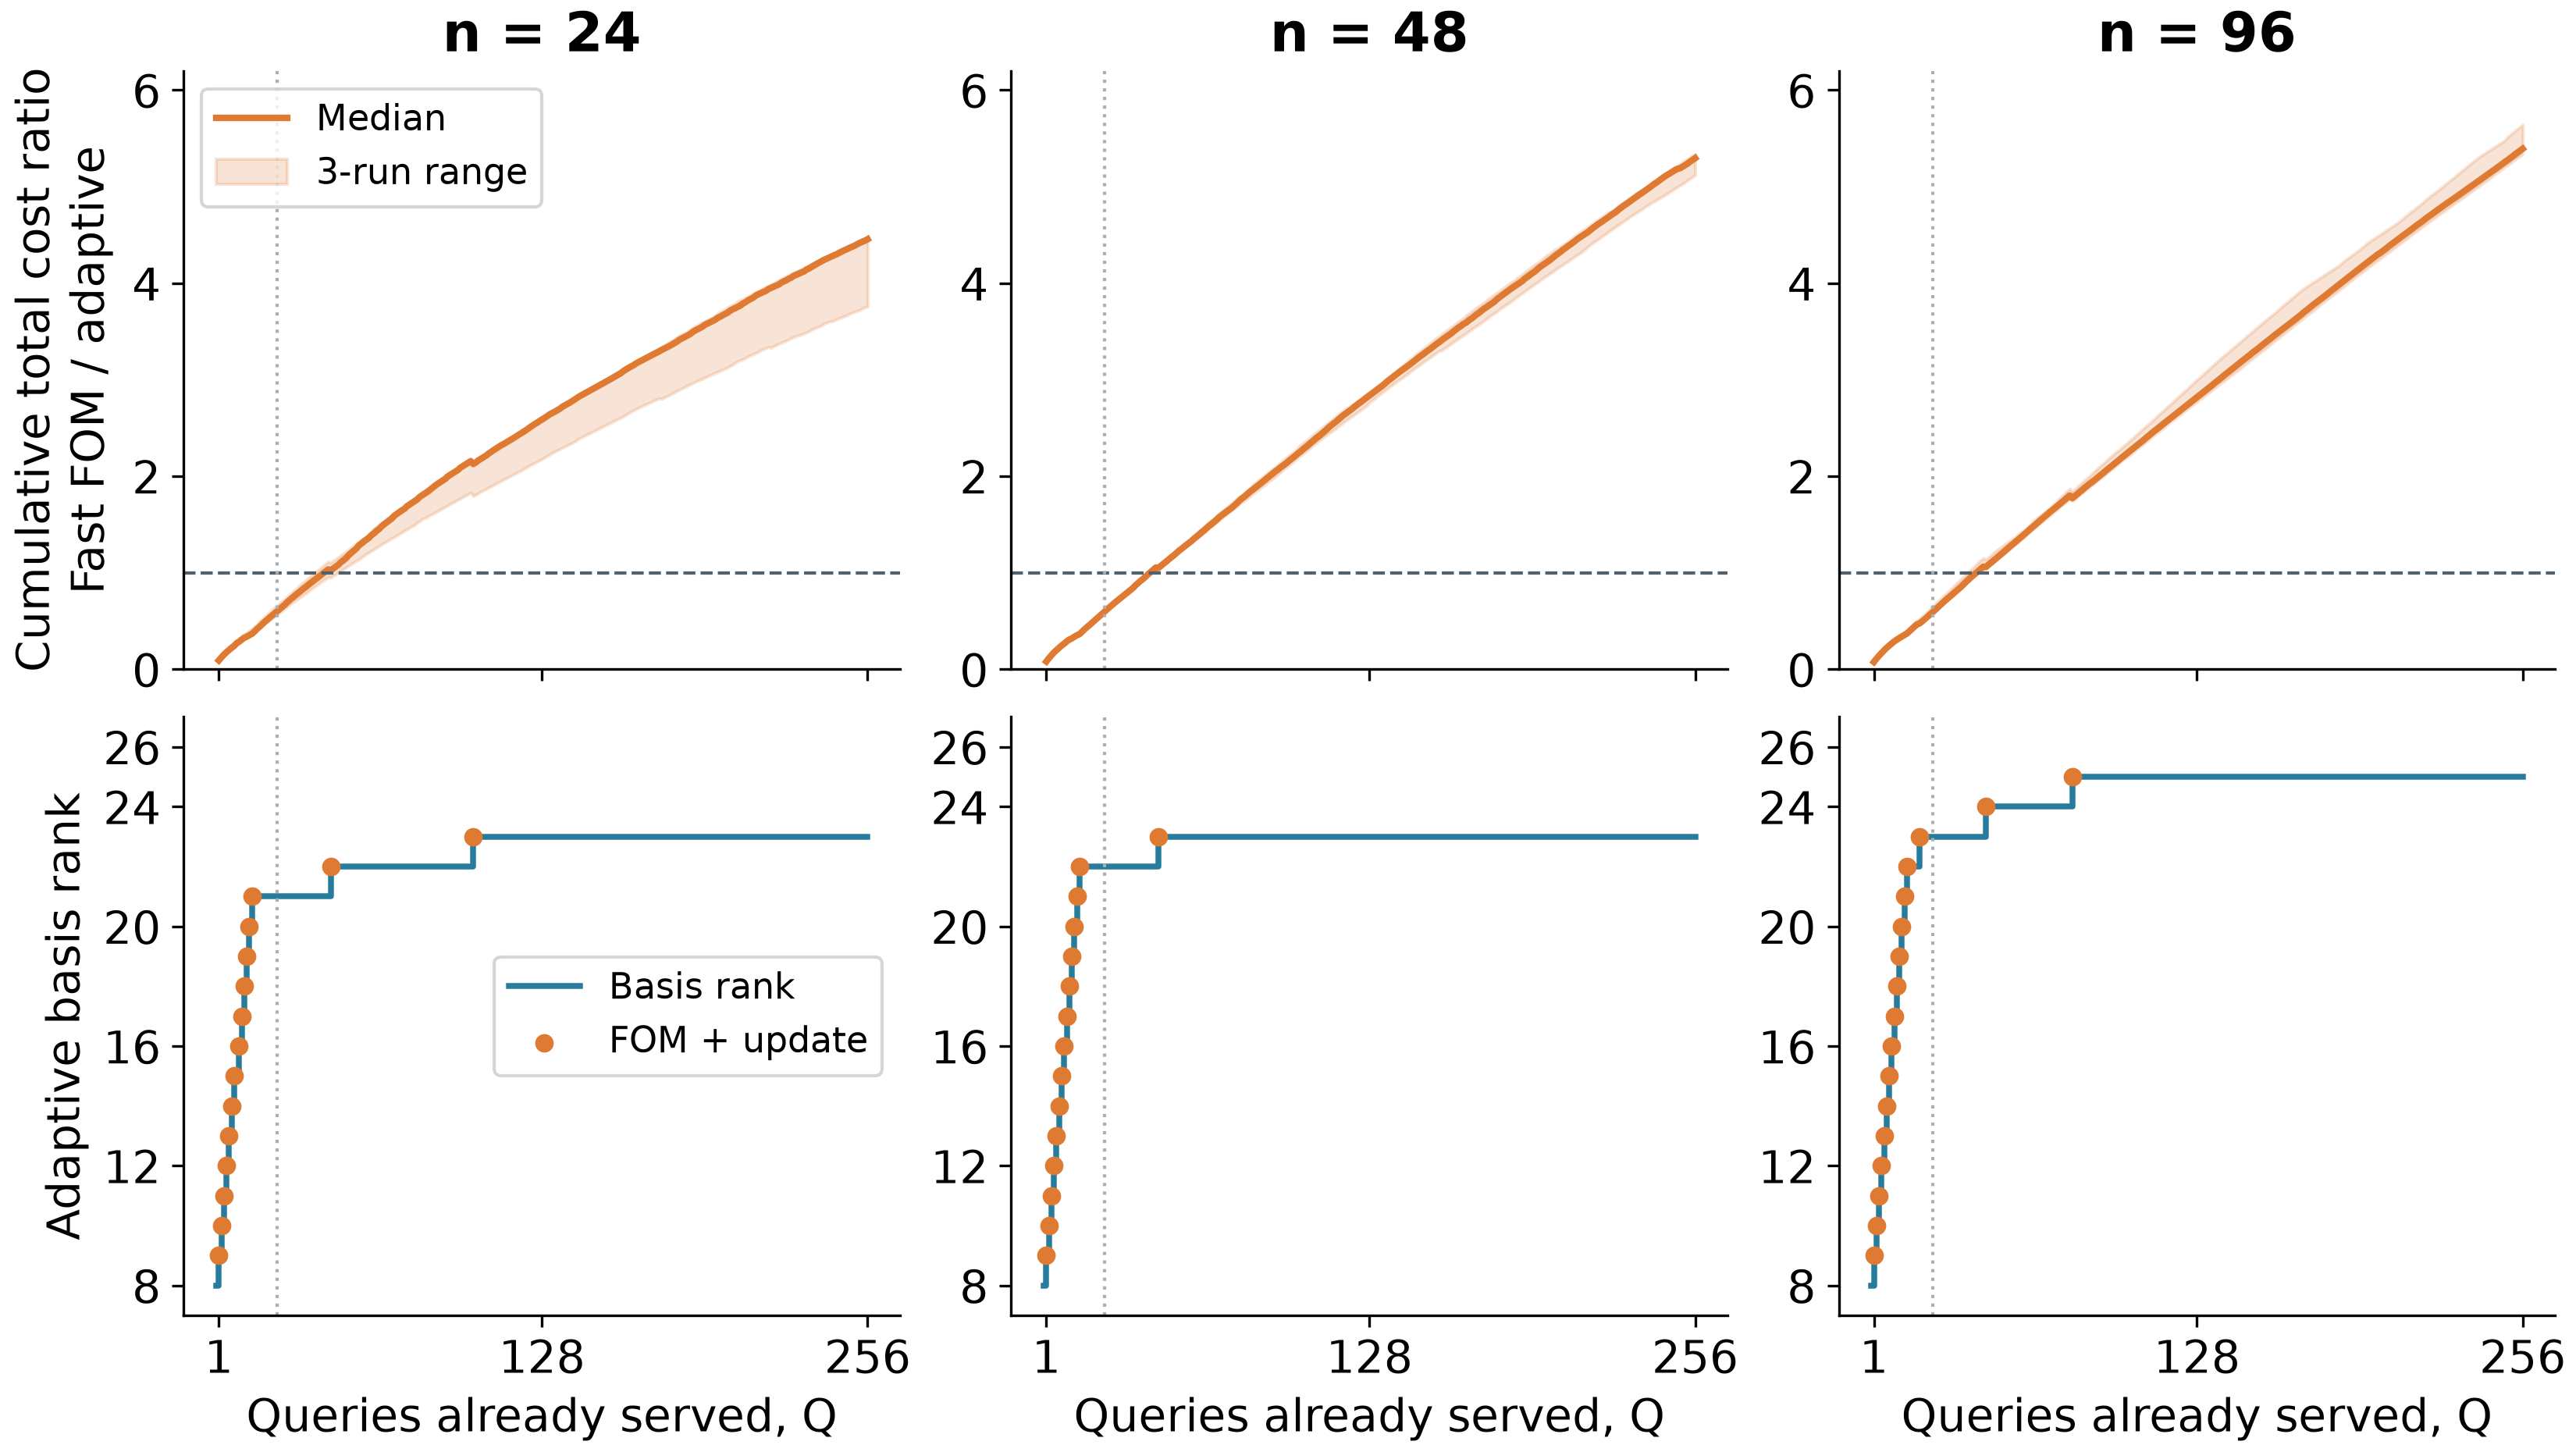
\includegraphics[width=0.94\linewidth]{figures/final_online_trace.png}
\caption{冻结参数流上的累计总成本比与基更新轨迹。阴影为三次计时的最小--最大范围，不是置信区间；竖虚线表示第 24 次查询。基更新轨迹在重复运行中一致。触发标记对应回退前的屏障判断，不能将回退后的误差当作触发准确性的依据。}
\label{fig:final-trace}
\end{figure}

\subsection{计入离线投入后的成本}
表\ref{tab:final-cost}使用前节定义的必要部署成本 $C_m$，以及以快速 FOM 为分子的总成本比 $S_m$。各列分别取三次重复的中位数；比值是\emph{逐次配对计算后再取中位数}，不要求等于两个耗时中位数的商。表内秒数不包含大模型研究、人工复核、报告制作和可选事后诊断。

\begin{table}[htbp]
\centering\small
\caption{五种方法的必要总成本（秒）及配对成本比中位数。$S>1$ 表示比快速 FOM 节省总成本。}
\label{tab:final-cost}
\begin{tabular}{rlrrrr}
\toprule
 & & \multicolumn{2}{c}{$Q=24$} & \multicolumn{2}{c}{$Q=256$}\\
\cmidrule(lr){3-4}\cmidrule(lr){5-6}
$n$ & 方法 & $C_m$ & $S_m$ & $C_m$ & $S_m$\\
\midrule
24 & 原始 FOM & 0.045281 & 0.456 & 0.508565 & 0.393\\
24 & 快速 FOM & 0.021096 & 1.000 & 0.201588 & 1.000\\
24 & 原始固定 POD & 0.047435 & 0.426 & 0.304257 & 0.666\\
24 & 快速固定 POD & 0.019477 & 1.004 & 0.023815 & 8.561\\
24 & 自适应 POD & 0.032453 & 0.603 & 0.045845 & 4.455\\
\midrule
48 & 原始 FOM & 0.171587 & 0.403 & 1.820013 & 0.395\\
48 & 快速 FOM & 0.069271 & 1.000 & 0.719447 & 1.000\\
48 & 原始固定 POD & 0.177342 & 0.398 & 1.166352 & 0.611\\
48 & 快速固定 POD & 0.071240 & 0.972 & 0.076377 & 9.304\\
48 & 自适应 POD & 0.115201 & 0.600 & 0.135209 & 5.295\\
\midrule
96 & 原始 FOM & 0.748842 & 0.460 & 8.197976 & 0.439\\
96 & 快速 FOM & 0.344734 & 1.000 & 3.543090 & 1.000\\
96 & 原始固定 POD & 0.763728 & 0.451 & 4.702765 & 0.753\\
96 & 快速固定 POD & 0.355942 & 0.969 & 0.363834 & 9.738\\
96 & 自适应 POD & 0.585963 & 0.588 & 0.657066 & 5.392\\
\bottomrule
\end{tabular}
\end{table}

\begin{table}[htbp]
\centering\small
\caption{自适应方案总成本比：中位数及三次计时的最小--最大范围。范围不是置信区间。}
\label{tab:final-ranges}
\begin{tabular}{rcc}
\toprule
$n$ & $Q=24$ & $Q=256$\\
\midrule
24 & $0.602599\;[0.570927,\,0.662752]$ & $4.455223\;[3.759159,\,4.461084]$\\
48 & $0.599792\;[0.599714,\,0.602662]$ & $5.294642\;[5.117985,\,5.339706]$\\
96 & $0.588320\;[0.579459,\,0.648001]$ & $5.392289\;[5.335244,\,5.640081]$\\
\bottomrule
\end{tabular}
\end{table}

短批量 $Q=24$ 时，自适应方案在三个网格上均未摊平离线成本；不能以在线服务加速替代这一结论。$Q=256$ 时，总成本比中位数约为 $4.46$--$5.39$，同时保持本次所有返回场达标。快速固定 $r=8$ POD 更省时，但存在场超标。原始固定 POD 的总成本比始终低于 1，说明低维求解本身不足以抵消重复组装与投影的开销。

\begin{figure}[htbp]
\centering
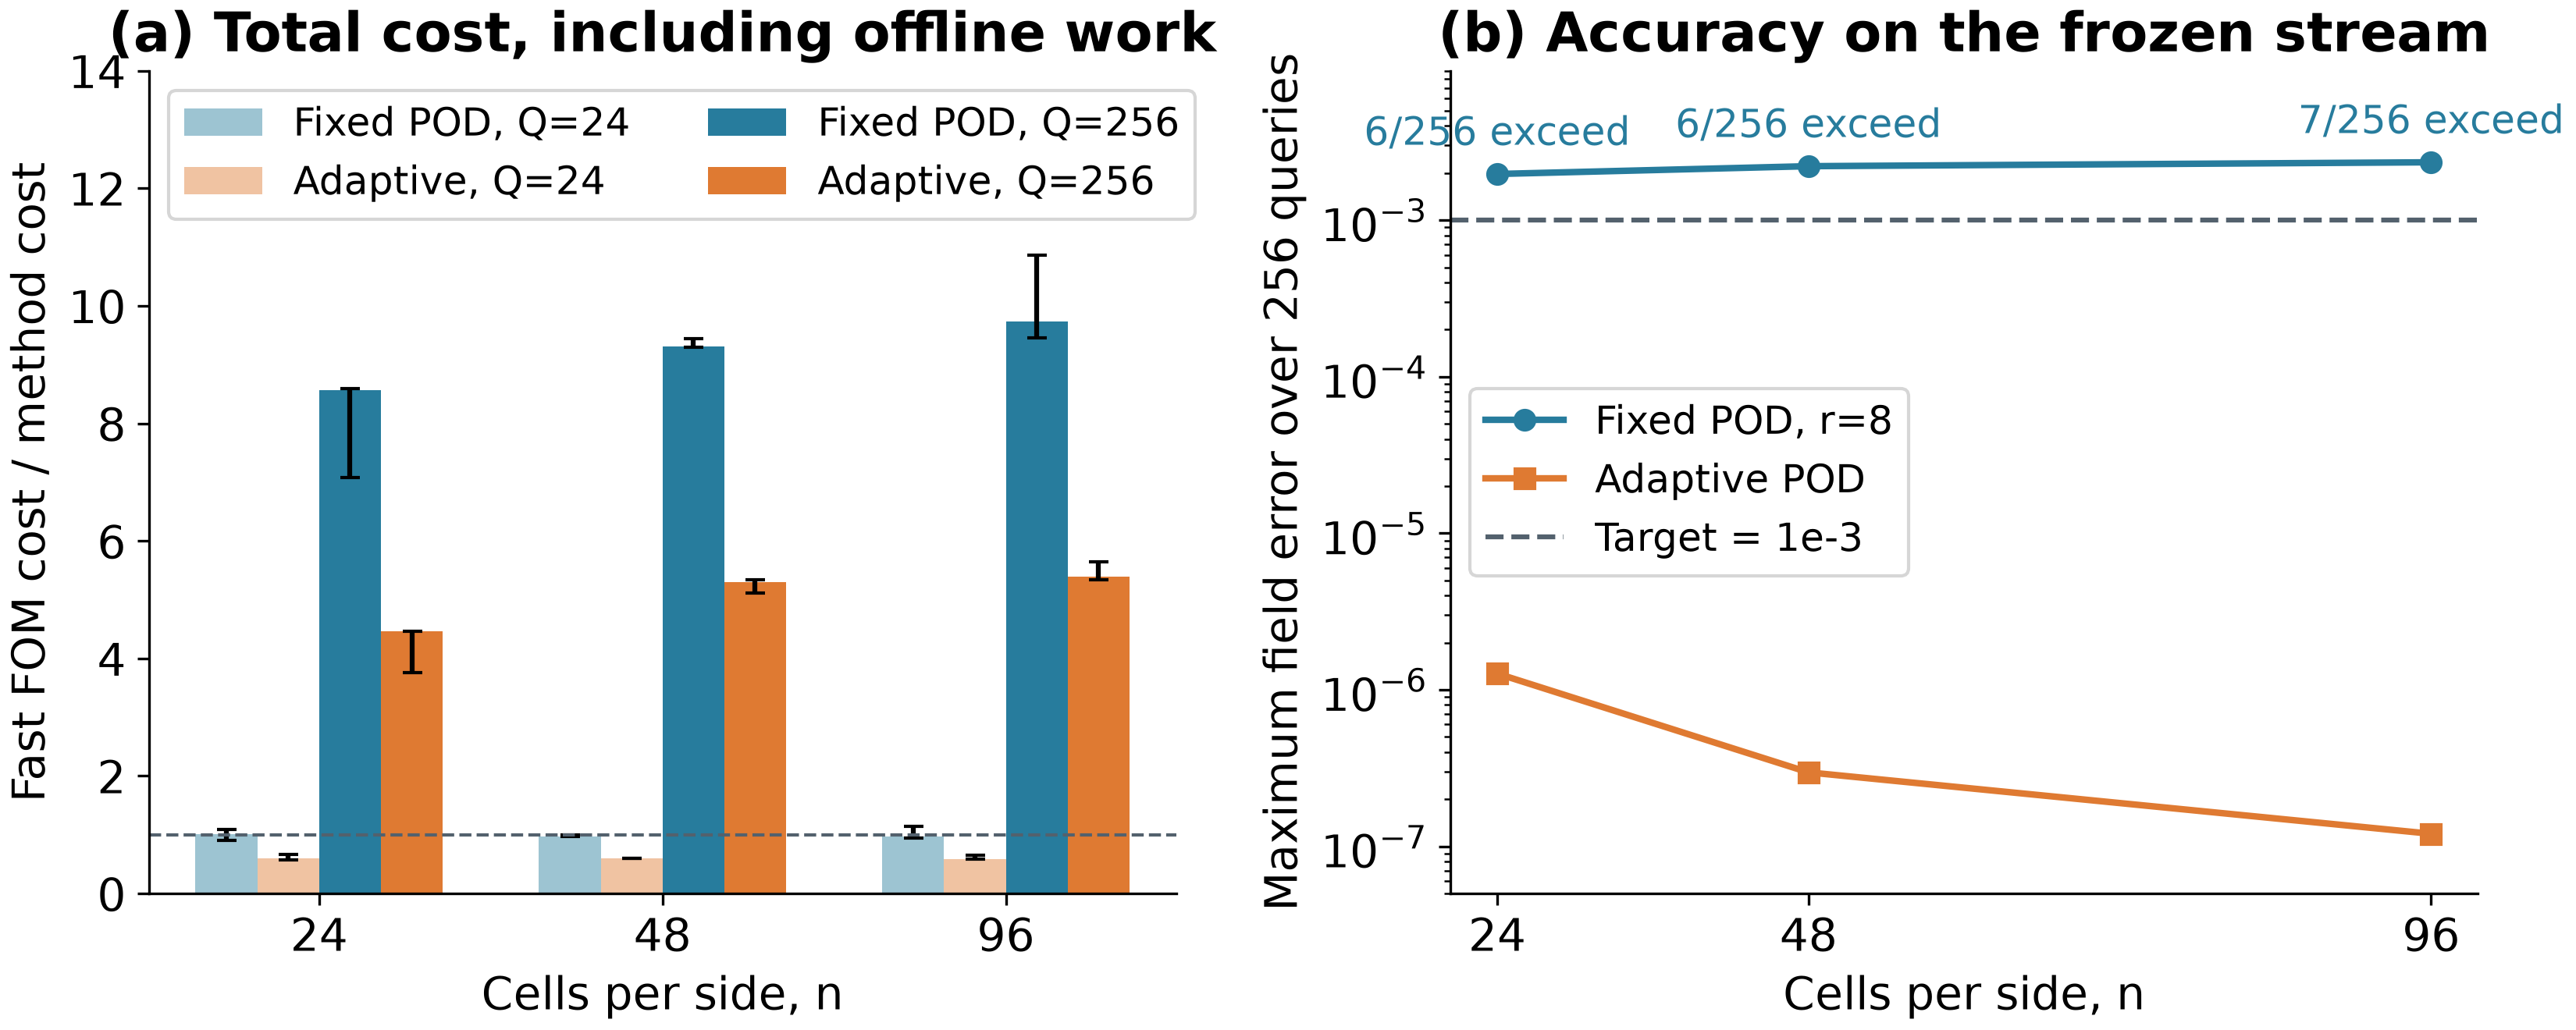
\includegraphics[width=0.94\linewidth]{figures/final_cost_accuracy.png}
\caption{最终精度与完整成本的联合比较。计时汇总基于同一参数序列的三次重复；所示最小--最大范围仅表示本机计时波动，不是置信区间，也不是新增精度样本。}
\label{fig:final-cost}
\end{figure}

运行环境为 Windows、Intel Core Ultra 9 275HX、约 63.38 GiB 内存，Python 3.12.14、NumPy 2.3.5、SciPy 1.18.1。线程环境变量请求单线程，但底层实际线程池规模未独立测量；桌面后台负载也未完全隔离。因此这些秒数和范围属于本机观测，不能外推为跨硬件性能保证。

\subsection{独立复核、完成范围与后续问题}
外部复核记录 \texttt{final\_crosscheck.json} 的 24 项检查全部通过，包含冻结顺序与摘要、九次运行及汇总记账、原生执行证据和独立数值复算。外部实际另做了 72 次训练 FOM、768 次参照 FOM、768 次固定 ROM、768 次自适应 ROM 及 47 次回退，按三个网格各复放一次相同参数流；这些工作不计入 Moonshine 原生调用次数或部署成本，也没有产生新的测试参数。场误差统计最大差为 $3.63\times10^{-15}$ 以下，指标差为 $2.81\times10^{-12}$ 以下，保存的最坏温度场差为 $3.56\times10^{-15}$ 以下。原生文件摘要保持不变。该复核是普通浮点程序证据，不是区间认证或形式化证明。

最终结果首次提交 Moonshine 审核时，计算与逻辑审核为正确，假设审核因材料未展开两个矩形热源的单元面积积分式而未能确定，整体未通过。后续补充源项定义及总热量 $\sum b_{ij}=0.12$ 后，原生综合审核通过；补证未改变算法、测试参数或数值结果，首次未定记录仍保留。该模型审核与外部程序复算是两条不同的证据链，均不能冒称形式化数学证明。

本研究已形成从离散模型、固定 POD 失效、解析屏障检查，到真实回退与基更新、冻结测试和成本复核的可追溯数值闭环。在本次有限合成参数流上，自适应方案以一定额外开销换取了较小的场误差，并在长查询批量中摊平离线投入；短批量失败和全部保守触发同样是研究结果。\textbf{最终协议没有比较固定 $r=24$ 等更强基线}，尽管已有 24 个训练快照，因此不能声称优于最优固定 ROM，也不能把本实验提升为工业热仿真问题已经解决。

下一步可检验的问题是：在同一独立部署成本和新增冻结测试下，增加固定基维数与收紧屏障估计，哪一种更有效地减少误触发和总耗时？连续 PDE 的离散误差、三维复杂结构、温度相关材料和非线性边界仍在本研究范围之外。解析屏障依托已有单调矩阵思想，由外部先验提供、经 Moonshine 检查和实现；本项目的价值在于实际研究过程及其可核验边界，而非宣称发现新的通用定理。
